\documentclass{article}
\usepackage[a4paper,left=3cm,right=3cm,top=3cm,bottom=3cm]{geometry}
\usepackage[utf8]{inputenc}
\usepackage[T1]{fontenc}
\usepackage{latexsym,amsfonts,amsmath,amssymb,amstext,graphicx,titlesec,ae,aecompl,mathtools,tabularx, multirow, cancel, nicefrac,subcaption, blindtext, floatrow}
\setlength{\parindent}{0pt}
\newfloatcommand{capbtabbox}{table}[][\FBwidth]


\begin{document}

\begin{titlepage}
       \begin{center}
             \begin{huge}
				   %% Update assignment number here
                   \textbf{Assignment 3}
             \end{huge}
       \end{center}

       \begin{center}
             \begin{large}
                   Computational Intelligence, SS2020
             \end{large}
       \end{center}

       \begin{center}
 \begin{tabularx}{\textwidth}{|>{\hsize=.33\hsize}X|>{\hsize=.33\hsize}X|>{\hsize=.33\hsize}X|} 

                   \hline
                   \multicolumn{3}{|c|}{\textbf{Team Members}} \\
                   \hline
                   Last name & First name & Matriculation Number \\
                   \hline
                   Blöcher & Christian & 01573246 \\
                   \hline
                   Bürgener & Max & 01531577 \\
                   \hline
                    &  &  \\
                   \hline

             \end{tabularx}
       \end{center}
\end{titlepage}

\section{Regression with Neural Networks}
\subsection{Simple Regression with Neural Networks}
\subsubsection{Learned Function}

Figure \ref{1_1_a} shows "typical" (slight variations occur due to non-fixed random seeds) results of functions learned through regression with $n_h = 2,5,50$ neurons in one hidden layer. Using only 2 neurons causes underfitting and leads to a poorly approximated function for both training and test sets. With $n_h=5$ yields better results for both training and testing sets, but especially for the testing set the approximated function is not entirely accurate. Choosing $n_h=50$ leads to overfitting: the output function fits the training data almost perfectly but barely resembles the testing set.

\begin{figure}[!ht]
\vspace*{-80pt}
\centering
\begin{subfigure}{0.78\textwidth}
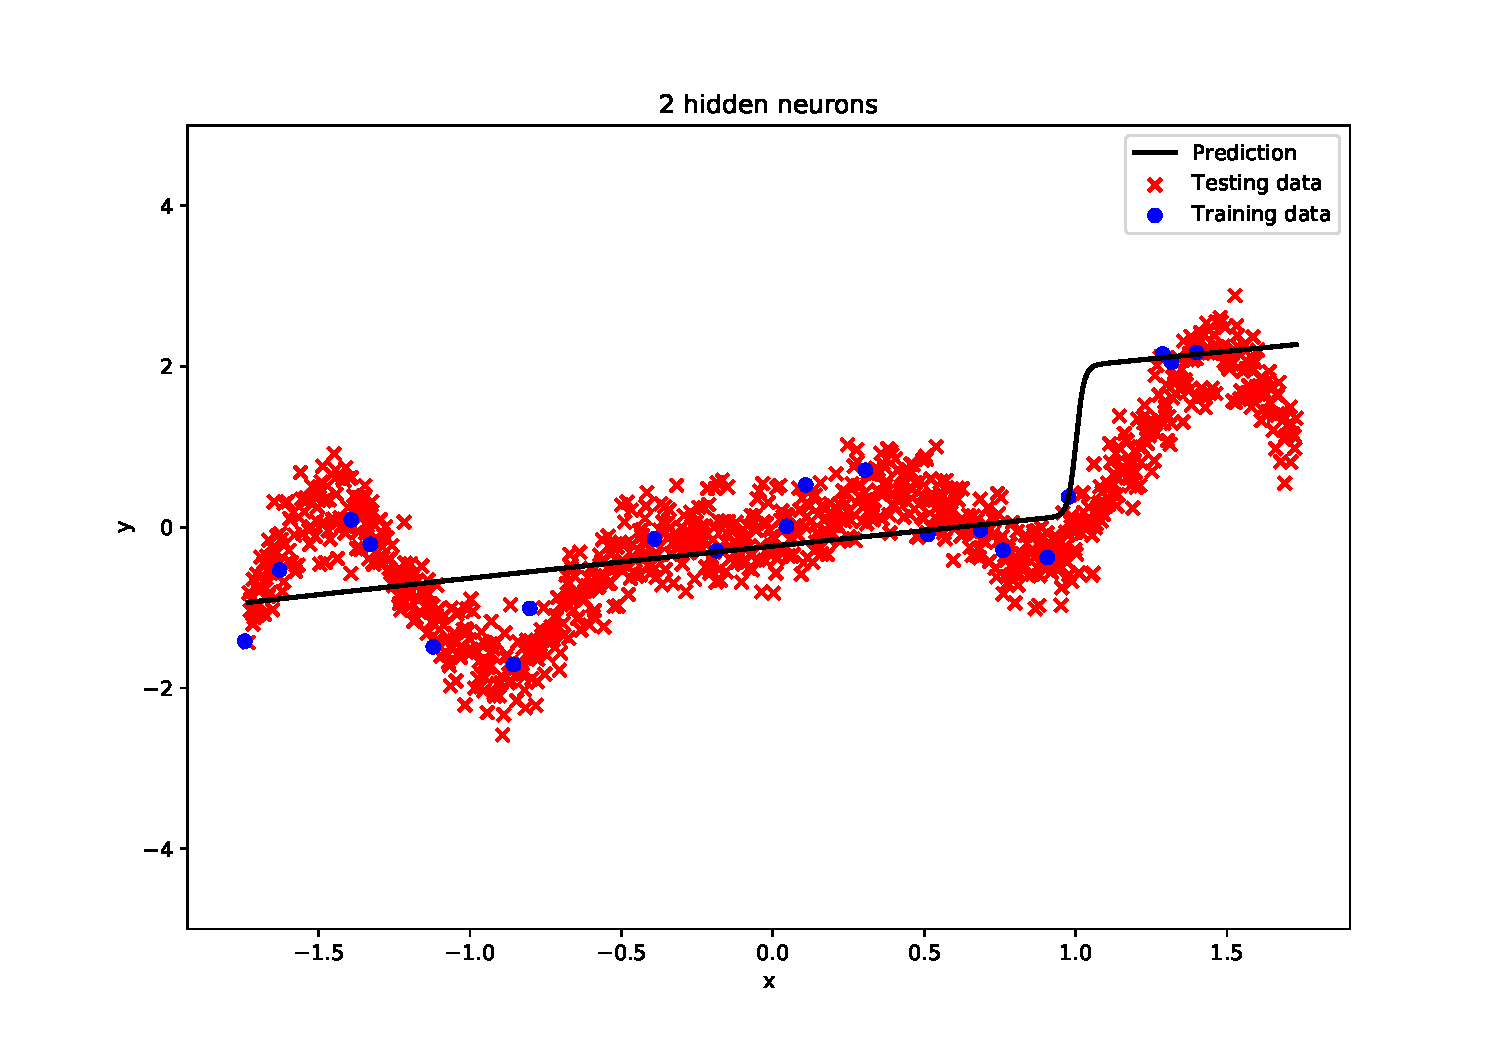
\includegraphics[width=\textwidth]{./Figures/1_1_a_nh_2.pdf}
\caption{$n_h=2$}
\end{subfigure}

\begin{subfigure}{0.78\textwidth}
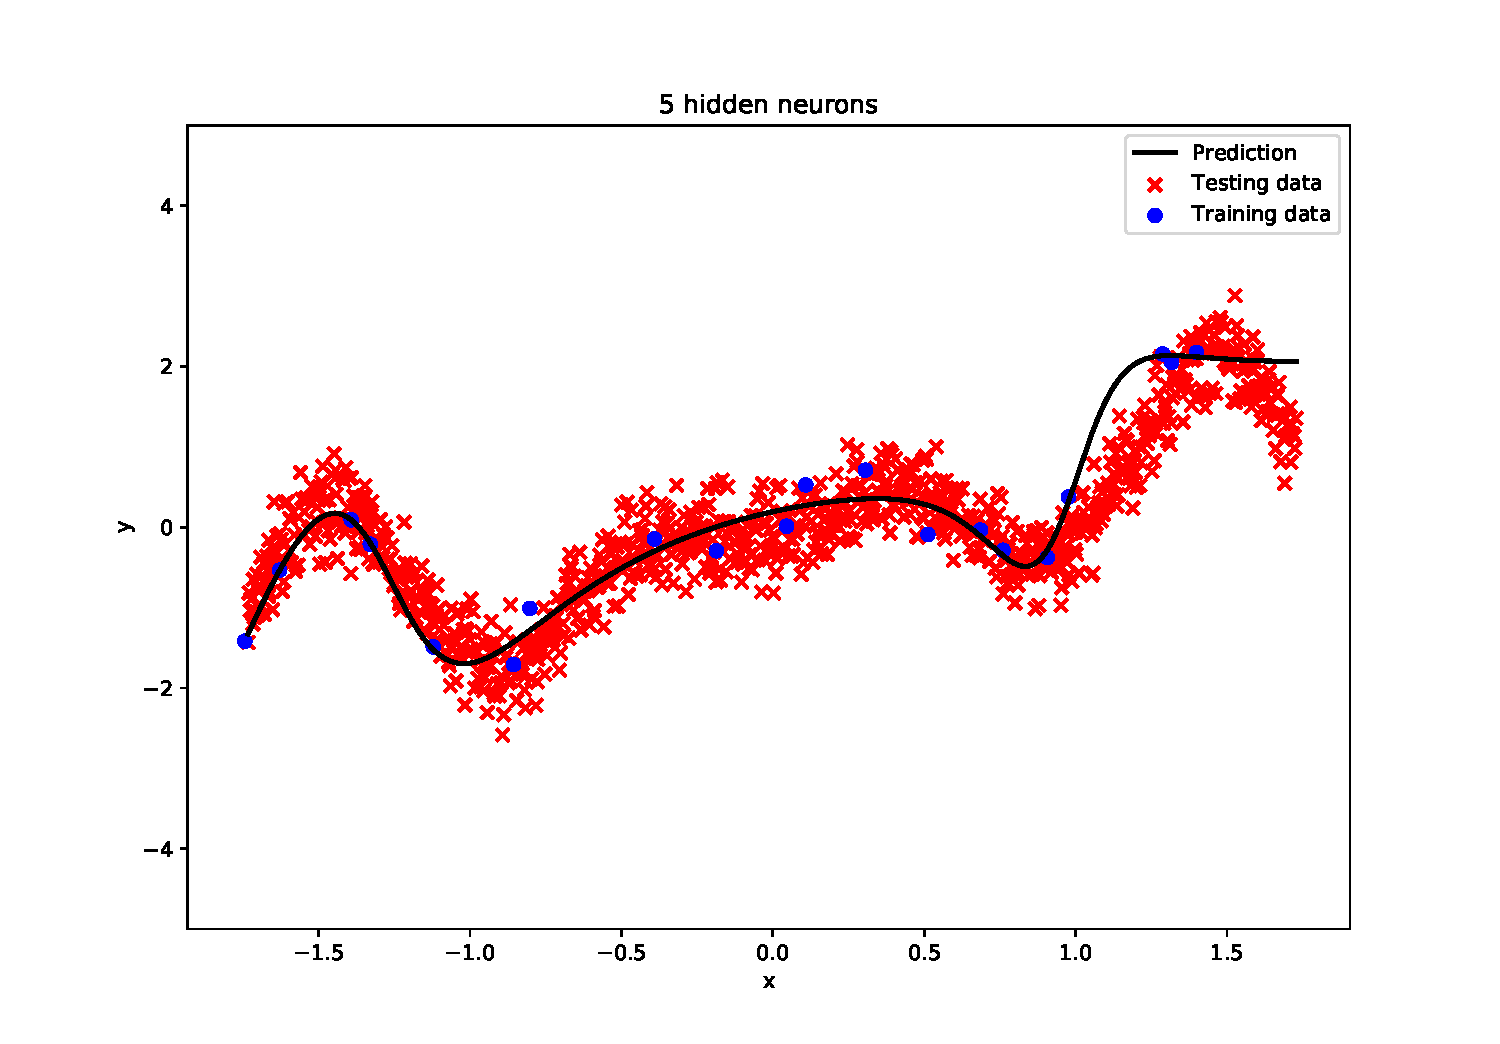
\includegraphics[width=\textwidth]{./Figures/1_1_a_nh_5.pdf}
\caption{$n_h=5$}
\end{subfigure}

\begin{subfigure}{0.78\textwidth}
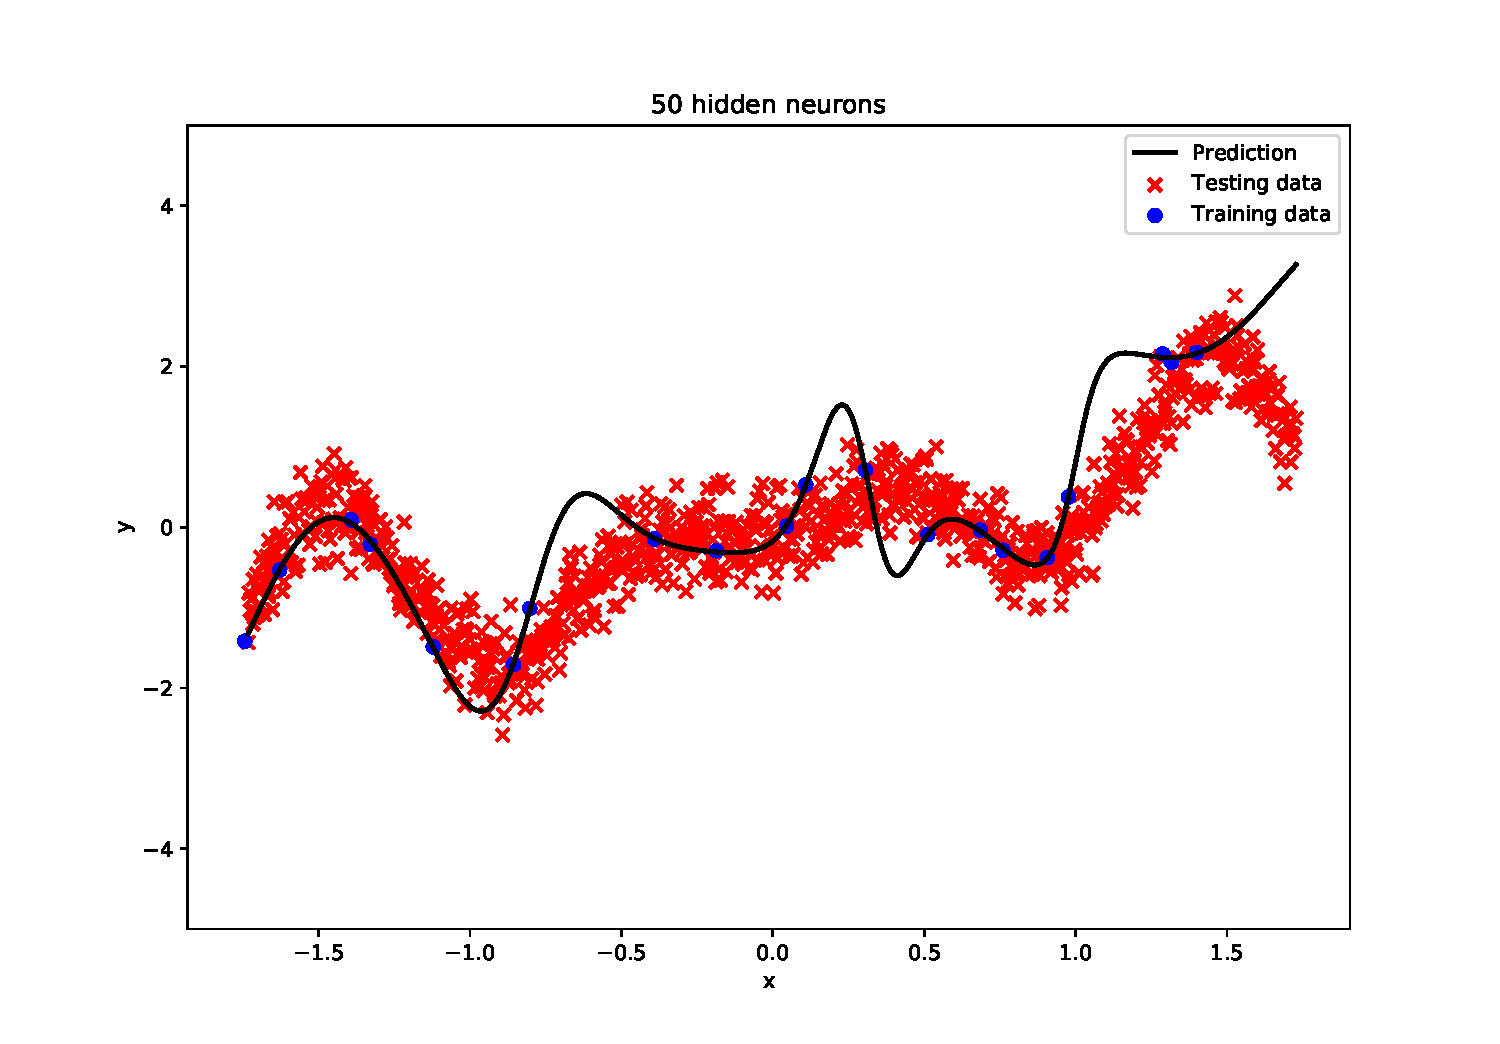
\includegraphics[width=\textwidth]{./Figures/1_1_a_nh_50.pdf}
\caption{$n_h=50$}
\end{subfigure}

\caption{Results of Regression with varying number of neurons $n_h$.}
\label{1_1_a}
\end{figure}


\subsubsection{Variability of the performance of deep neural networks}

Table \ref{1_1_b} shows the minimum, maximum, mean, and standard deviation of the MSE obtained on the training set for $n_h=5$ and seeds $0 \dots 9$. The minimum MSE on the training set is achieved with seed $3$, for the testing set however the best seed is $7$. With a validation set one could run the fitting process for multiple seeds, then choose the seed with the smallest MSE on the validation set. Now that the risk of overfitting has been reduced it is possible to make a better prediction on the testing set.\\
The variability of the MSE across seeds is expected, because a non-linear activation function (sigmoid $\sigma(x)$) is used. This causes the cost function to have multiple (local) minima instead of just one global minimum. Which of the minima the algorithm converges on depends on the random weight initialization, leading to different MSEs. This occurs for both SGD and standard GD. Another source of randomness introduced by SGD is linked to its weight update: instead of using all training samples for each weight update only one randomly chosen sample is used for each update. That means SGD typically needs more iterations to converge because the path to the minimum is not as direct as with GD, but because only one sample is used per iteration the computational cost is greatly reduced, leading to faster training.

\begin{table}[!ht]
\centering
\begin{tabular}{|c|c|c|c|} \hline
min & max 	& $\mu$ 	& $\sigma$ \\ \hline
0.032	& 0.263		& 0.153		& 0.068  \\ \hline
\end{tabular}
\caption{Minimum, maximum, mean, and standard deviation of training set MSEs with $n_h=5$.}
\label{1_1_b}
\end{table}


\subsubsection{Varying the number of hidden neurons}

Figure \ref{1_1_c_mse} shows the mean and standard deviation of the MSEs for both training and test data. There are two notable peaks in the testing MSE at $n_h=6$ and $n_h=12$, which are caused by discontinuities or large peaks in the approximated functions between training samples (e.g. s. figure \ref{1_1_c_worst} for worst learned function with $n_h=6$) and which will be disregarded further on. With increasing number of hidden neurons the training cost decreases, as the training data gets better approximated. This leads to underfitting and a higher testing MSE for small values of $n_h$. The best result on the testing set averaged over the runs with different random seeds is achieved with $n_h=4$ (s. figure \ref{1_1_c_best} for best learned function with $n_h=4$). For larger values of $n_h$ the testing cost increases again due to overfitting.

\begin{figure}[!ht]
\centering
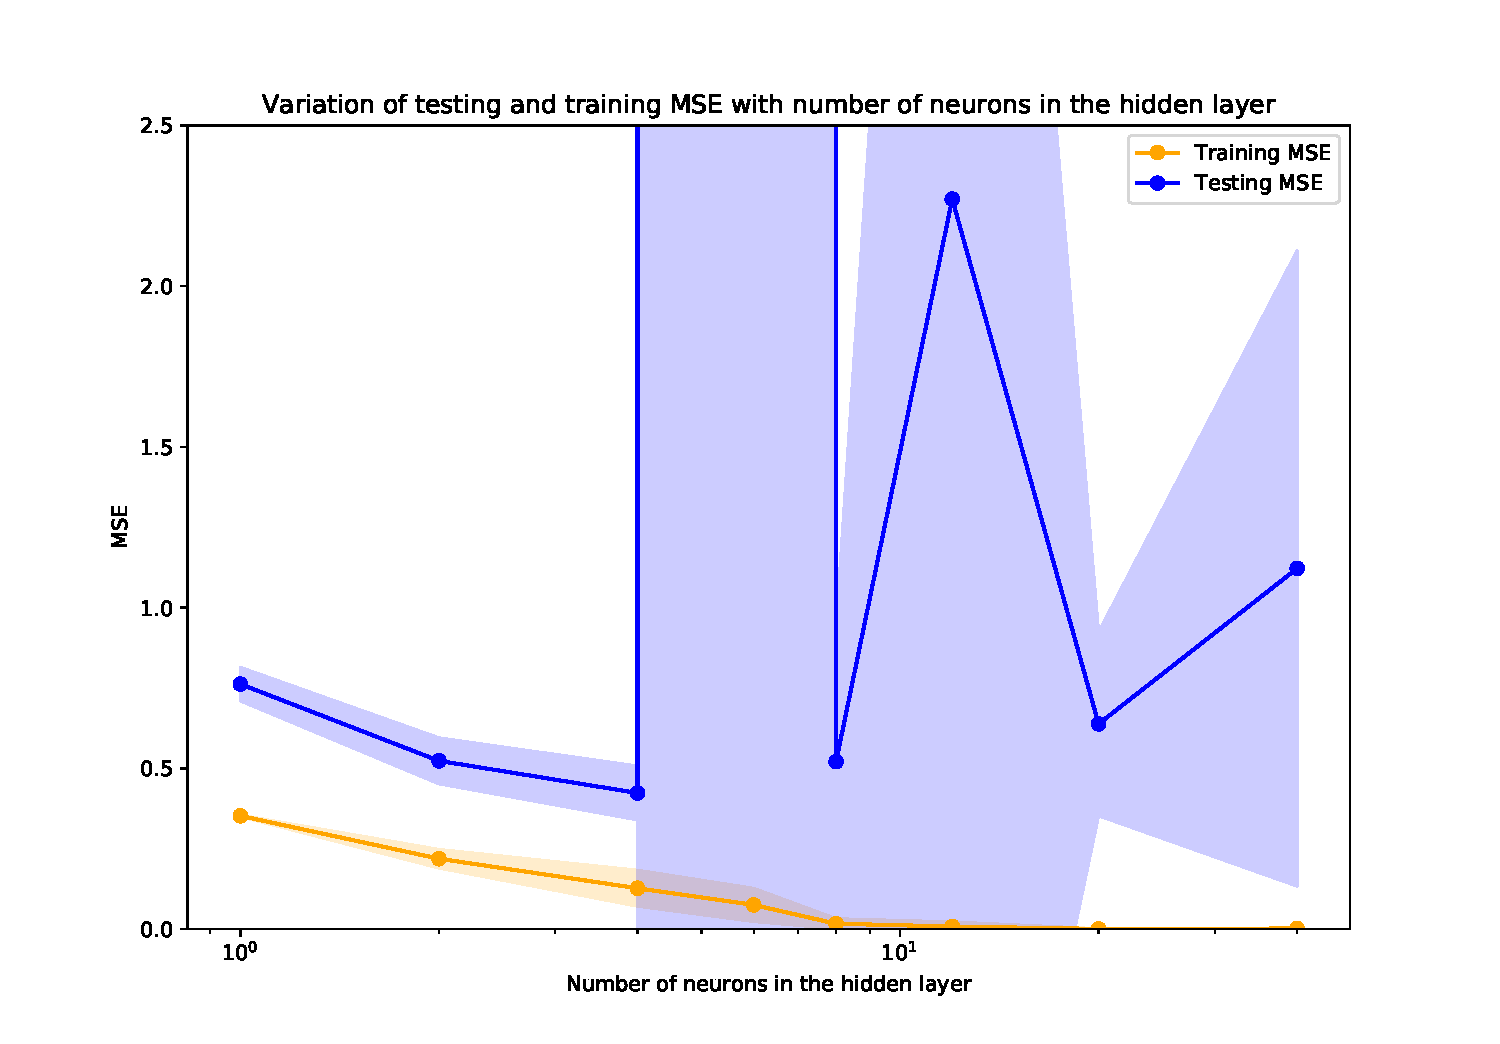
\includegraphics[width=\textwidth]{./Figures/1_1_c_mse.pdf}
\caption{Variation of testing and training MSE for varying $n_h$.}
\label{1_1_c_mse}
\end{figure}

\begin{figure}[!ht]
\centering
\begin{subfigure}{0.8\textwidth}
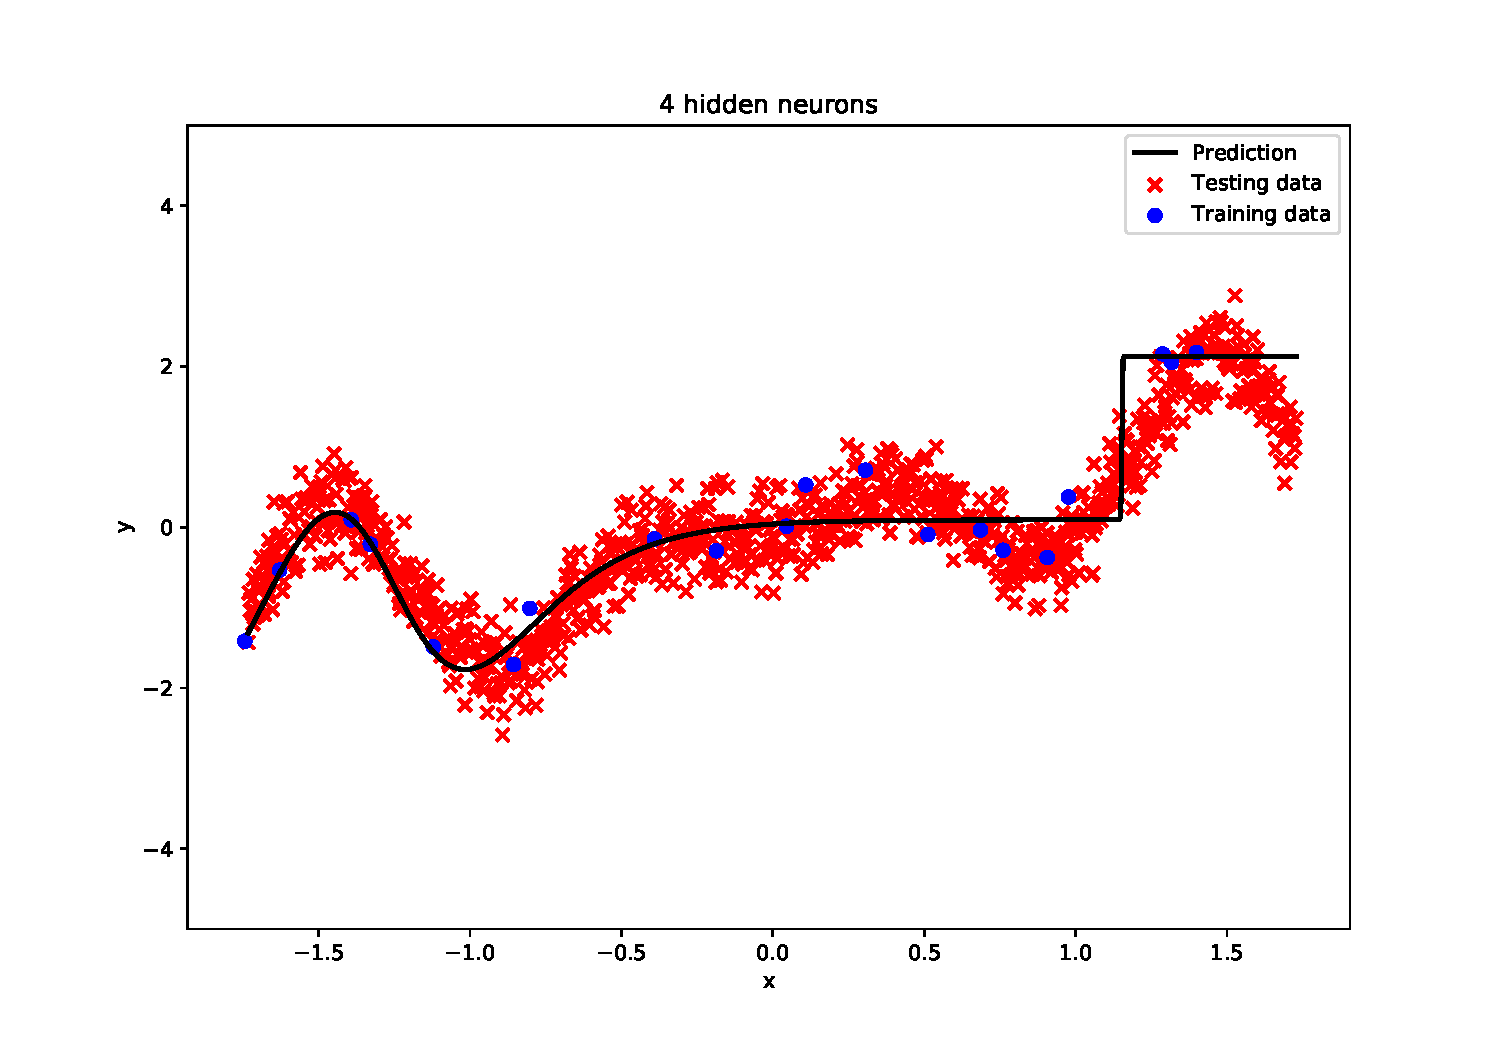
\includegraphics[width=\textwidth]{./Figures/1_1_c_nh_besttest.pdf}
\caption{Best result: $n_h=4$}
\label{1_1_c_best}
\end{subfigure}

\begin{subfigure}{0.8\textwidth}
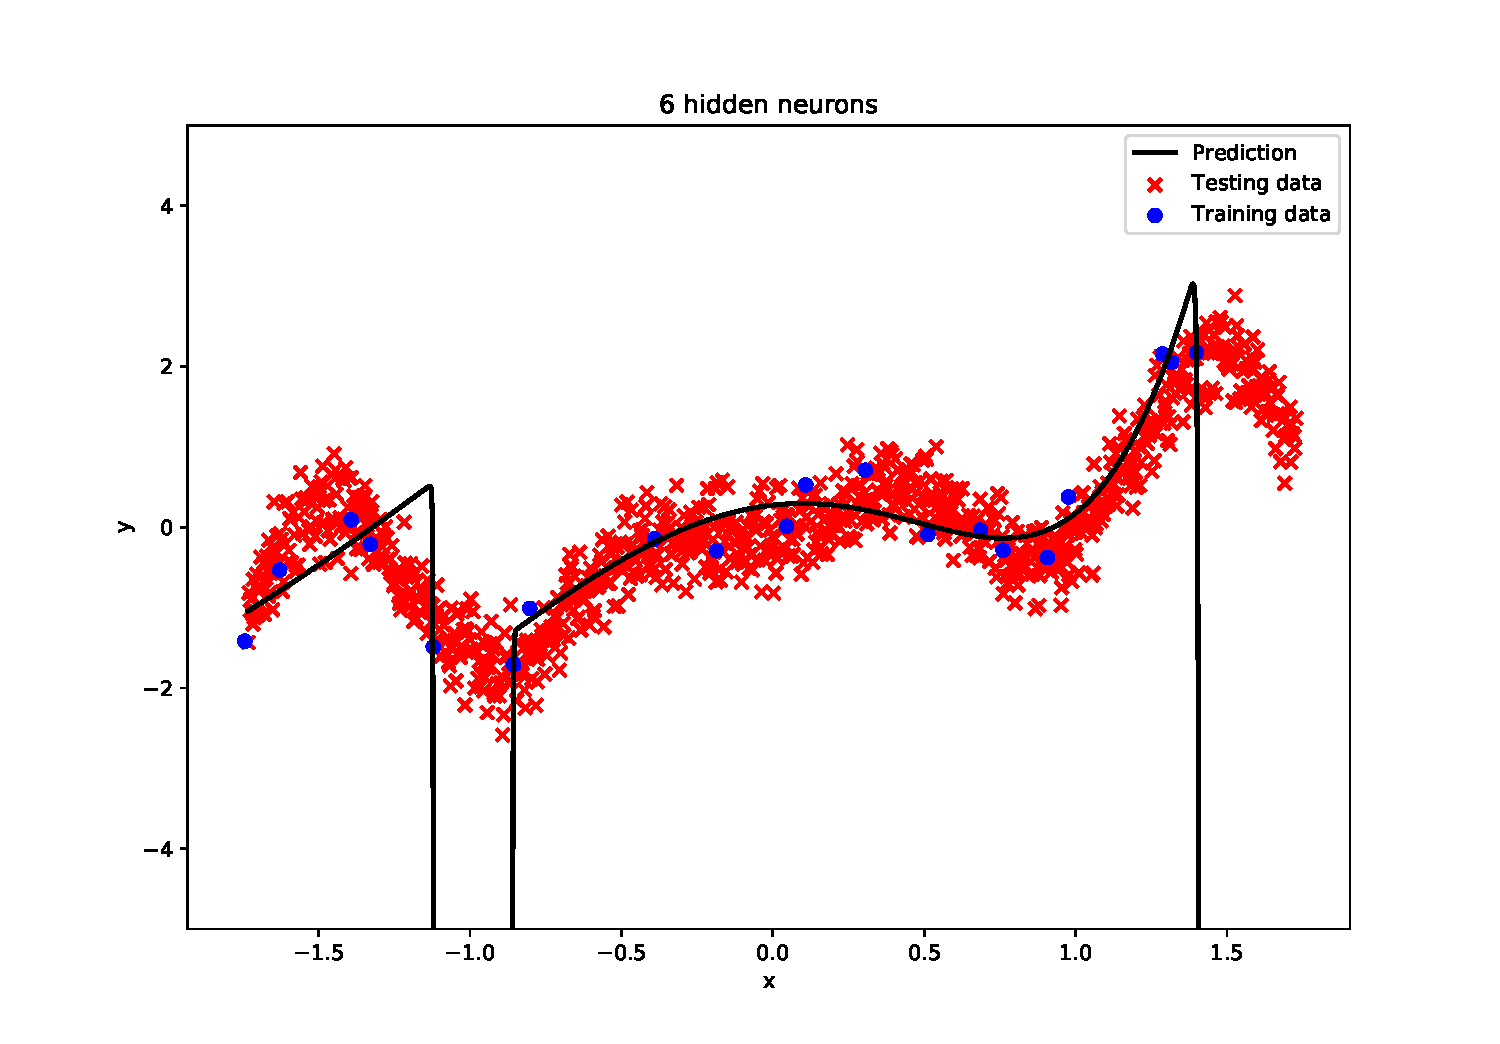
\includegraphics[width=\textwidth]{./Figures/1_1_c_nh_worsttest.pdf}
\caption{Worst result: $n_h=6$}
\label{1_1_c_worst}
\end{subfigure}

\caption{Best and worst result of regression with varying $n_h$.}
\label{1_1_c_bestworst}
\end{figure}

\subsubsection{Change of MSE during the course of training}

Figure \ref{1_1_d_mse} shows the MSE during the course of training for $n_h=2,5,50$. Because of the random initialization all maximum MSEs for training and testing data are at the very beginning of the update loop. As the weights get fitted on the training data all training MSEs decrease subsequently and converge at around $0.2$, $0.05$, and $0.3$ respectively. After an initial drop the testing MSEs rise to a local maximum again, which is reached the faster the smaller $n_h$. Then the testing MSEs decrease again until they converge at around $0.37$, $0.23$, and $0.5$ respectively, making $n_h=5$ the best number of hidden neurons. As the testing MSE is the largest with $n_h=50$ the risk of overfitting increases with the number of hidden neurons.\\
By using the SGD one can reduce overfitting: the random selection of the samples for the weight update causes the path to the minimum of the cost function to be noisy. Additionally by reducing the computational cost one can increase the size of the training set, which generally reduces the risk of overfitting.

\begin{figure}[!ht]
\centering
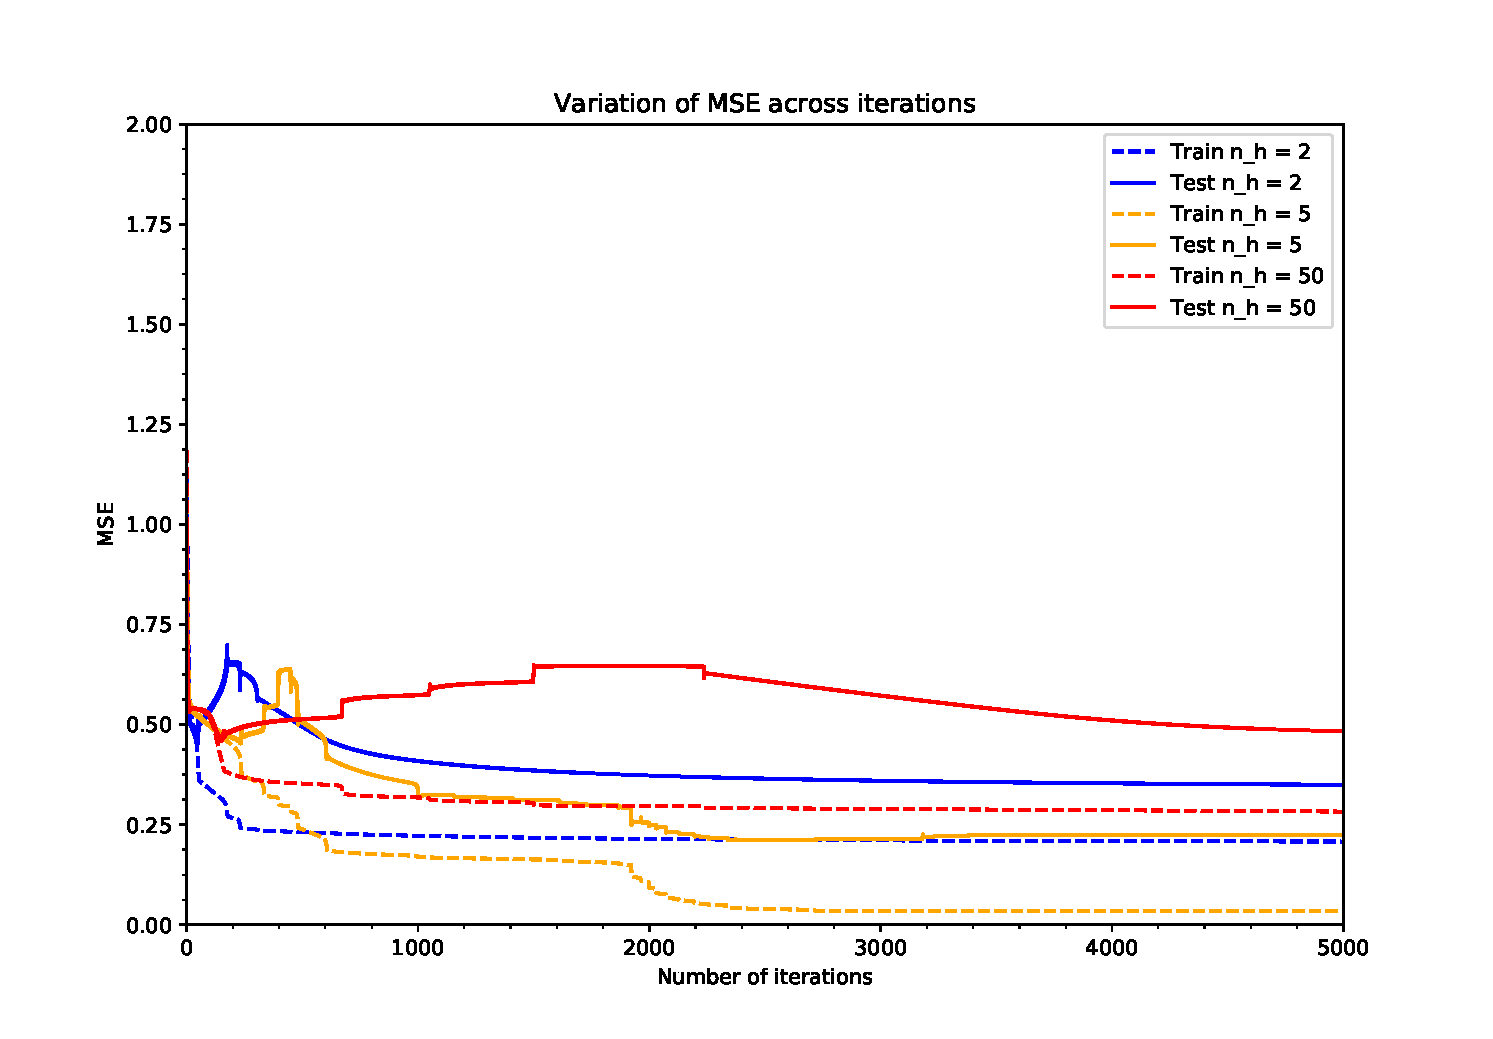
\includegraphics[width=\textwidth]{./Figures/1_1_d_mse.pdf}
\caption{Variation of testing and training MSE across iterations with varying $n_h$.}
\label{1_1_d_mse}
\end{figure}

\clearpage
\subsection{Regularized Neural Networks: Weight Decay}

\begin{figure}[!ht]
\centering
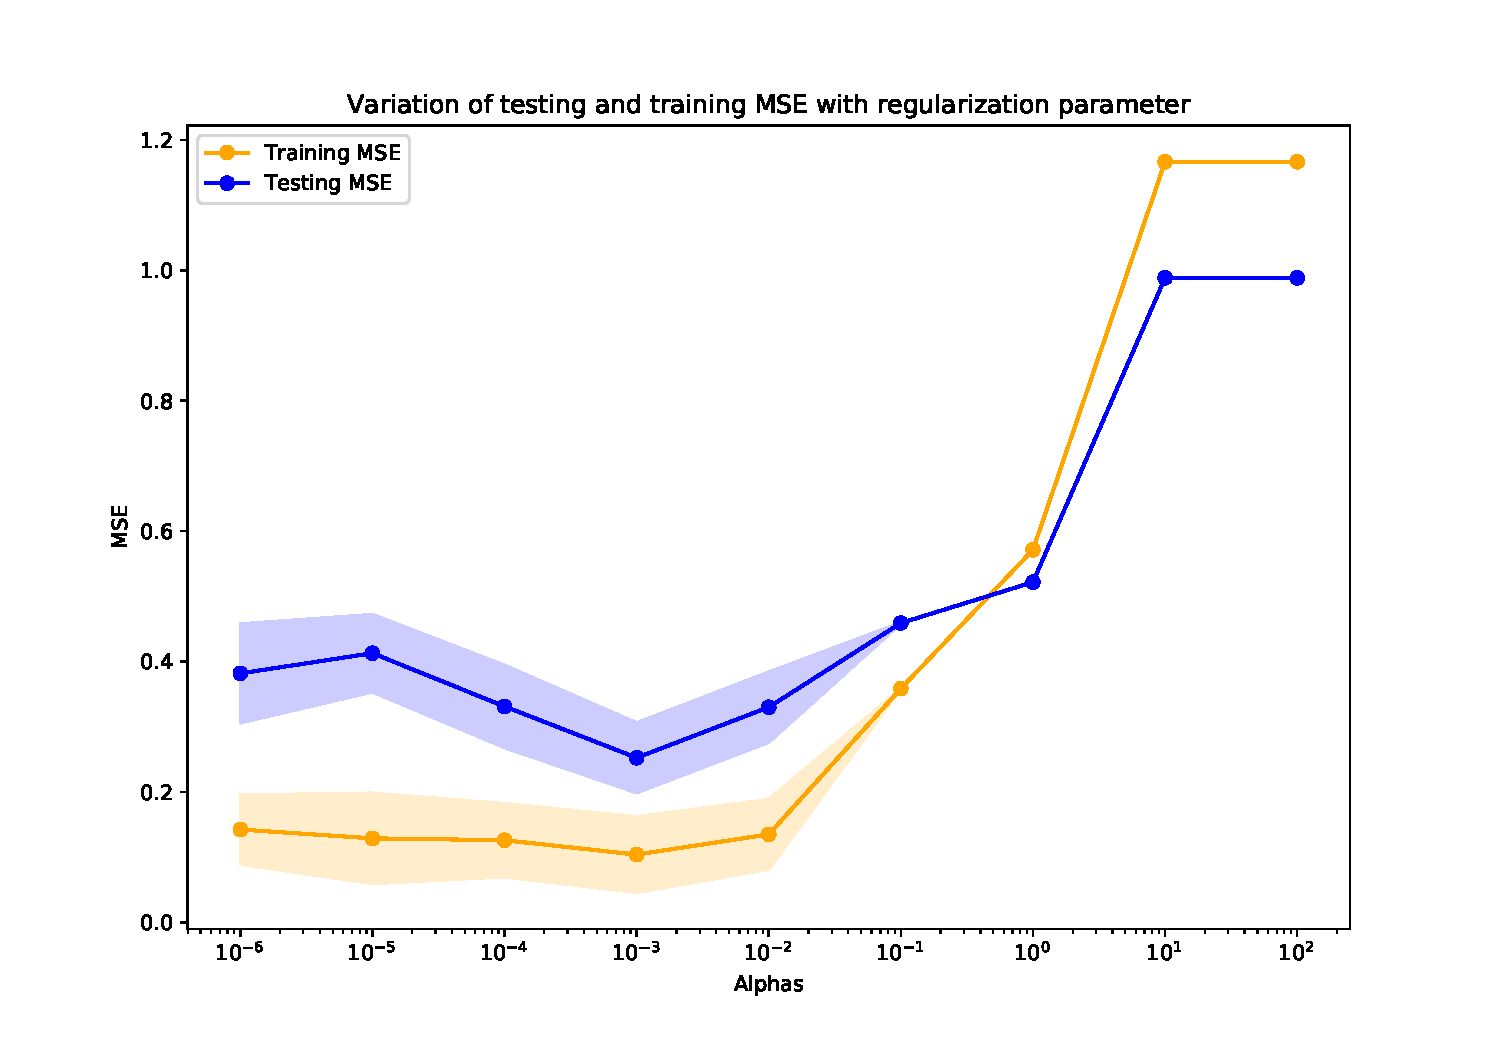
\includegraphics[width=\textwidth]{./Figures/1_2_mse.pdf}
\caption{Variation of testing and training MSE with regularization parameter $\alpha$.}
\label{1_2_mse}
\end{figure}

\clearpage
\section{Classification with Neural Networks: Fashion MNIST}

% Confusion matrix

\begin{table}[!ht]
\centering
      \begin{tabular}{|l||c|c|c|c|c|c|c|c|c|c|}
      \hline
                  & T-Shirt/top & Trousers & Pullover & Dress & Coat & Sandal & Shirt & Sneaker & Bag & Ankle boot \\ \hline \hline
      T-Shirt/top & 841         & 3        & 12       & 25    & 4    & 1      & 108   & 0       & 6   & 0          \\ \hline
      Trousers    & 7           & 960      & 2        & 21    & 5    & 0      & 4     & 0       & 1   & 0          \\ \hline
      Pullover    & 19          & 0        & 835      & 15    & 52   & 0      & 78    & 0       & 1   & 0          \\ \hline
      Dress       & 21          & 4        & 14       & 904   & 23   & 0      & 31    & 0       & 3   & 0          \\ \hline
      Coat        & 2           & 1        & 104      & 30    & 797  & 0      & 65    & 0       & 1   & 0          \\ \hline
      Sandal      & 1           & 0        & 0        & 1     & 0    & 955    & 0     & 23      & 2   & 18         \\ \hline
      Shirt       & 104         & 1        & 75       & 26    & 45   & 1      & 741   & 0       & 7   & 0          \\ \hline
      Sneaker     & 0           & 0        & 0        & 0     & 0    & 15     & 0     & 958     & 0   & 27         \\ \hline
      Bag         & 5           & 0        & 5        & 6     & 2    & 3      & 4     & 4       & 970 & 1          \\ \hline
      Ankle boot  & 1           & 0        & 0        & 0     & 0    & 9      & 0     & 3       & 0   & 960        \\ \hline
      \end{tabular}
      \end{table}

\clearpage
\section{Bonus: Implementation of a Perceptron}

\end{document}